\section{Projektmanagement}

\begin{figure}[h!]
	\centering
	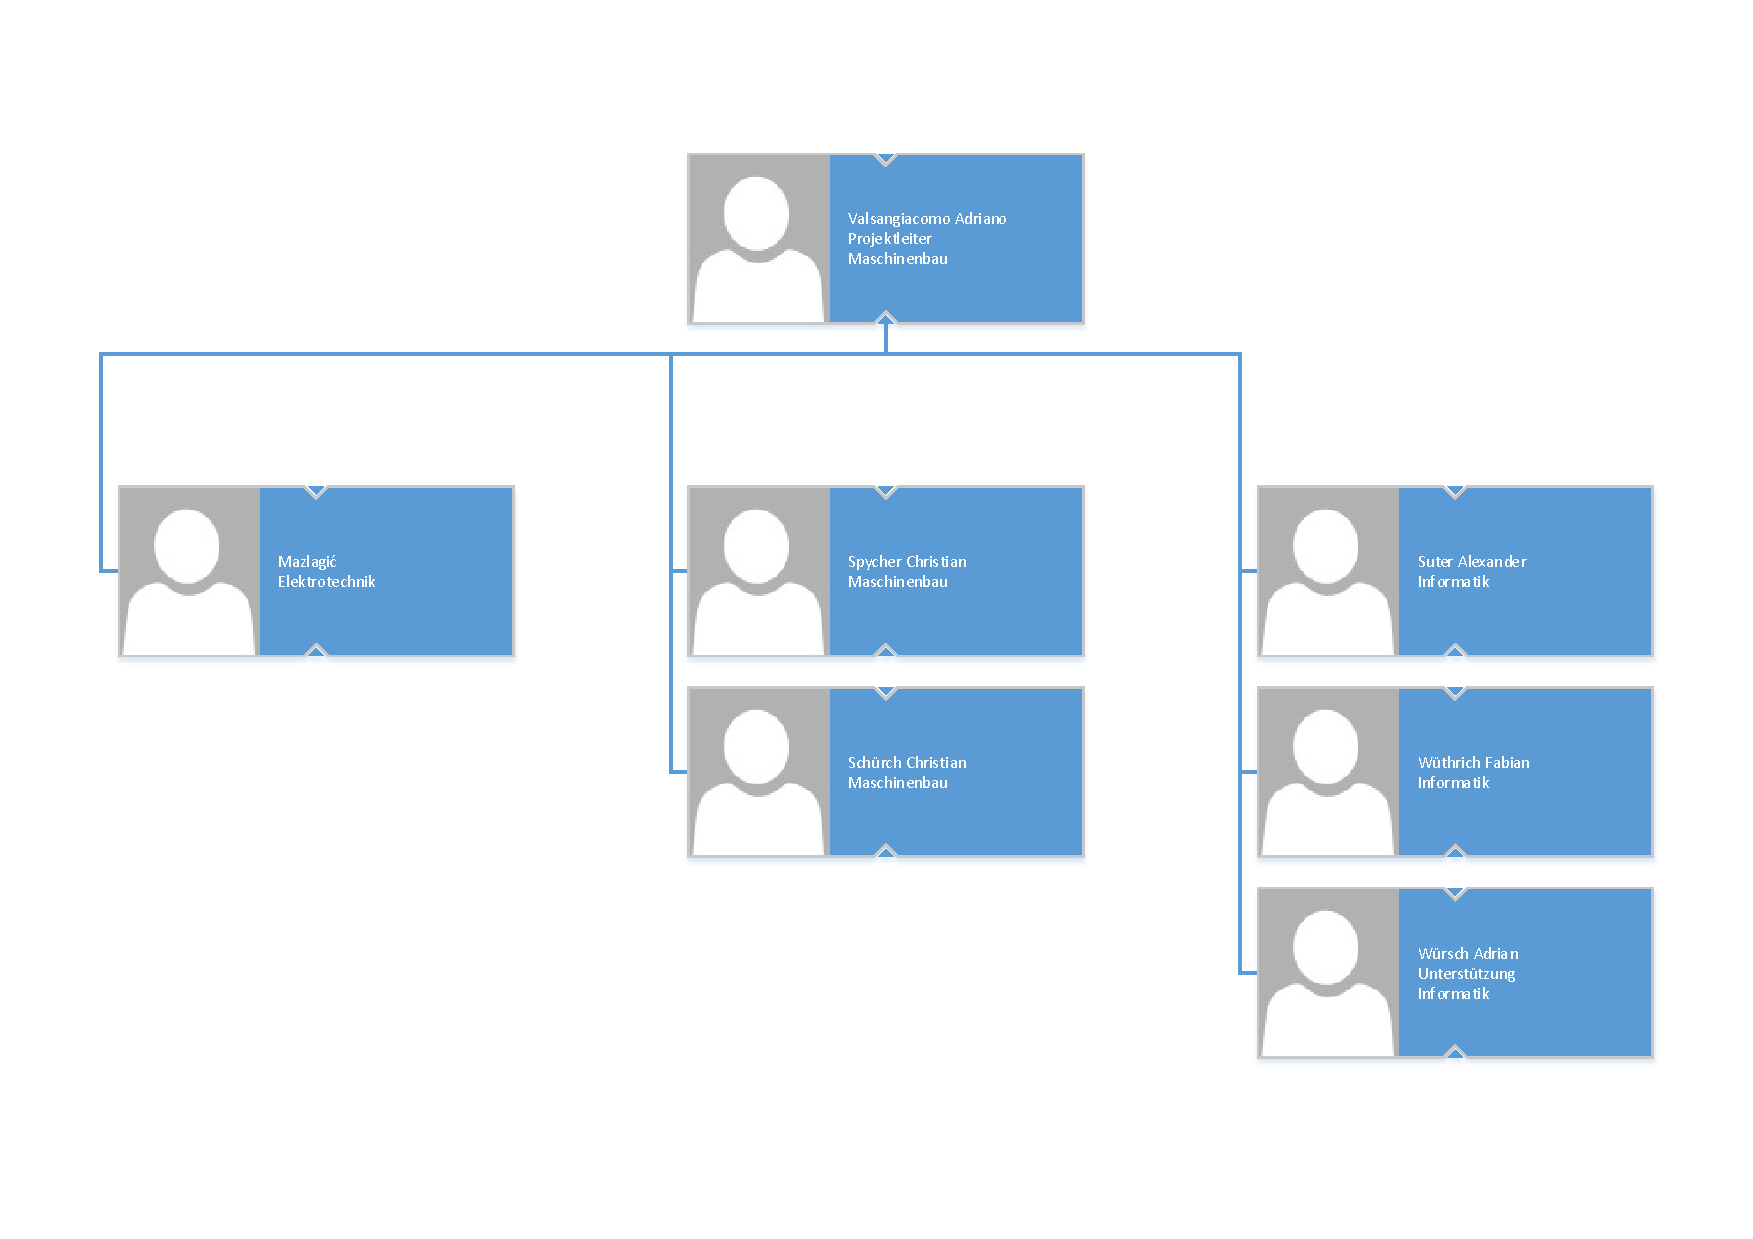
\includegraphics[width=1.0\linewidth]{../../fig/Organigramm.pdf}
	\caption{Organisation der Gruppe}
	\label{fig:Organigramm}
\end{figure}

\noindent
Die Projektführung wurde von Adriano Valsangiacomo durchgeführt. Er
koordinierte die einzelnen Teilgruppen und sorgte für reibungslosen
Betrieb. Fürs PREN2 hat das Team agile Verstärkung erhalten in Person von Adrian Würsch.

\newpage
\subsection{Grobplanung}
In der Grobplanung wurden die wichtigsten Meilensteine des Gesamtsystems und der einzelnen Disziplinen festgehalten.
Der Zeitstrahl in Abbildung \ref{fig:rahmenplanung} zeigt die chronologische Reihenfolge an. Als klar wurde, dass die Umsetzung in Verzug war, wurde die Planung angepasst. Vorallem im Bereich der Elektrotechnik wurde der Engpass ersichtlich. Wir waren uns bewusst, dass es dort zu Verzögerungen kommen kann, da dieser Bereich mehr oder weniger eine one-man-show ist. Darum wurden im ET Bereich zuerst Arbeiten erledigt, welche Abhängigkeiten mit anderen Disziplinen hatten.

\subsubsection{Stand 19.02.2015}
Der Rahmenplanung sind die wichtigsten Termine zu entnehmen. Dies sind drei offizielle Termine wie diverse kleinere, welche jeweils von den Disziplinen selbst für sich gesetzt wurden. Der erste Meilenstein wurde auf den 6. März datiert, dort soll sich das Team über die Planung und Umsetzung sicher sein.
Meilenstein zwei wurde auf den 10. April festgelegt, mit dem Ziel die Maschine fertig montiert zu haben. Eine Woche später sollte anschliessend die Tests beginnen. Die lauffähige und getestete Maschine und zugleich 80\% der Dokumentation bildeten zusammen Meilenstein 3.

\begin{figure}[h!]
	\centering
	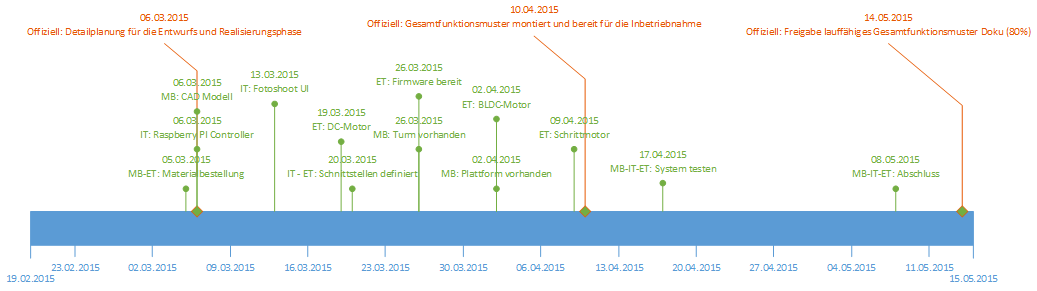
\includegraphics[width=1\linewidth]{../../fig/rahmenplanung}
	\caption{Rahmenplan vom 19.02.2015}
	\label{fig:rahmenplanung}
\end{figure}

\newpage
\subsubsection{Stand: 10.04.2015}
Am 10.04.2015 hat sich das Team zusammengeschlossen um über die restlichen Arbeiten zu diskutieren. Darauf hin hat man sich entschlossen die restliche Planung anzupassen. Nun wurden teilweise neue Termine definiert, welche für den restlichen Verlauf bindend sind.

\begin{figure}[h!]
	\centering
	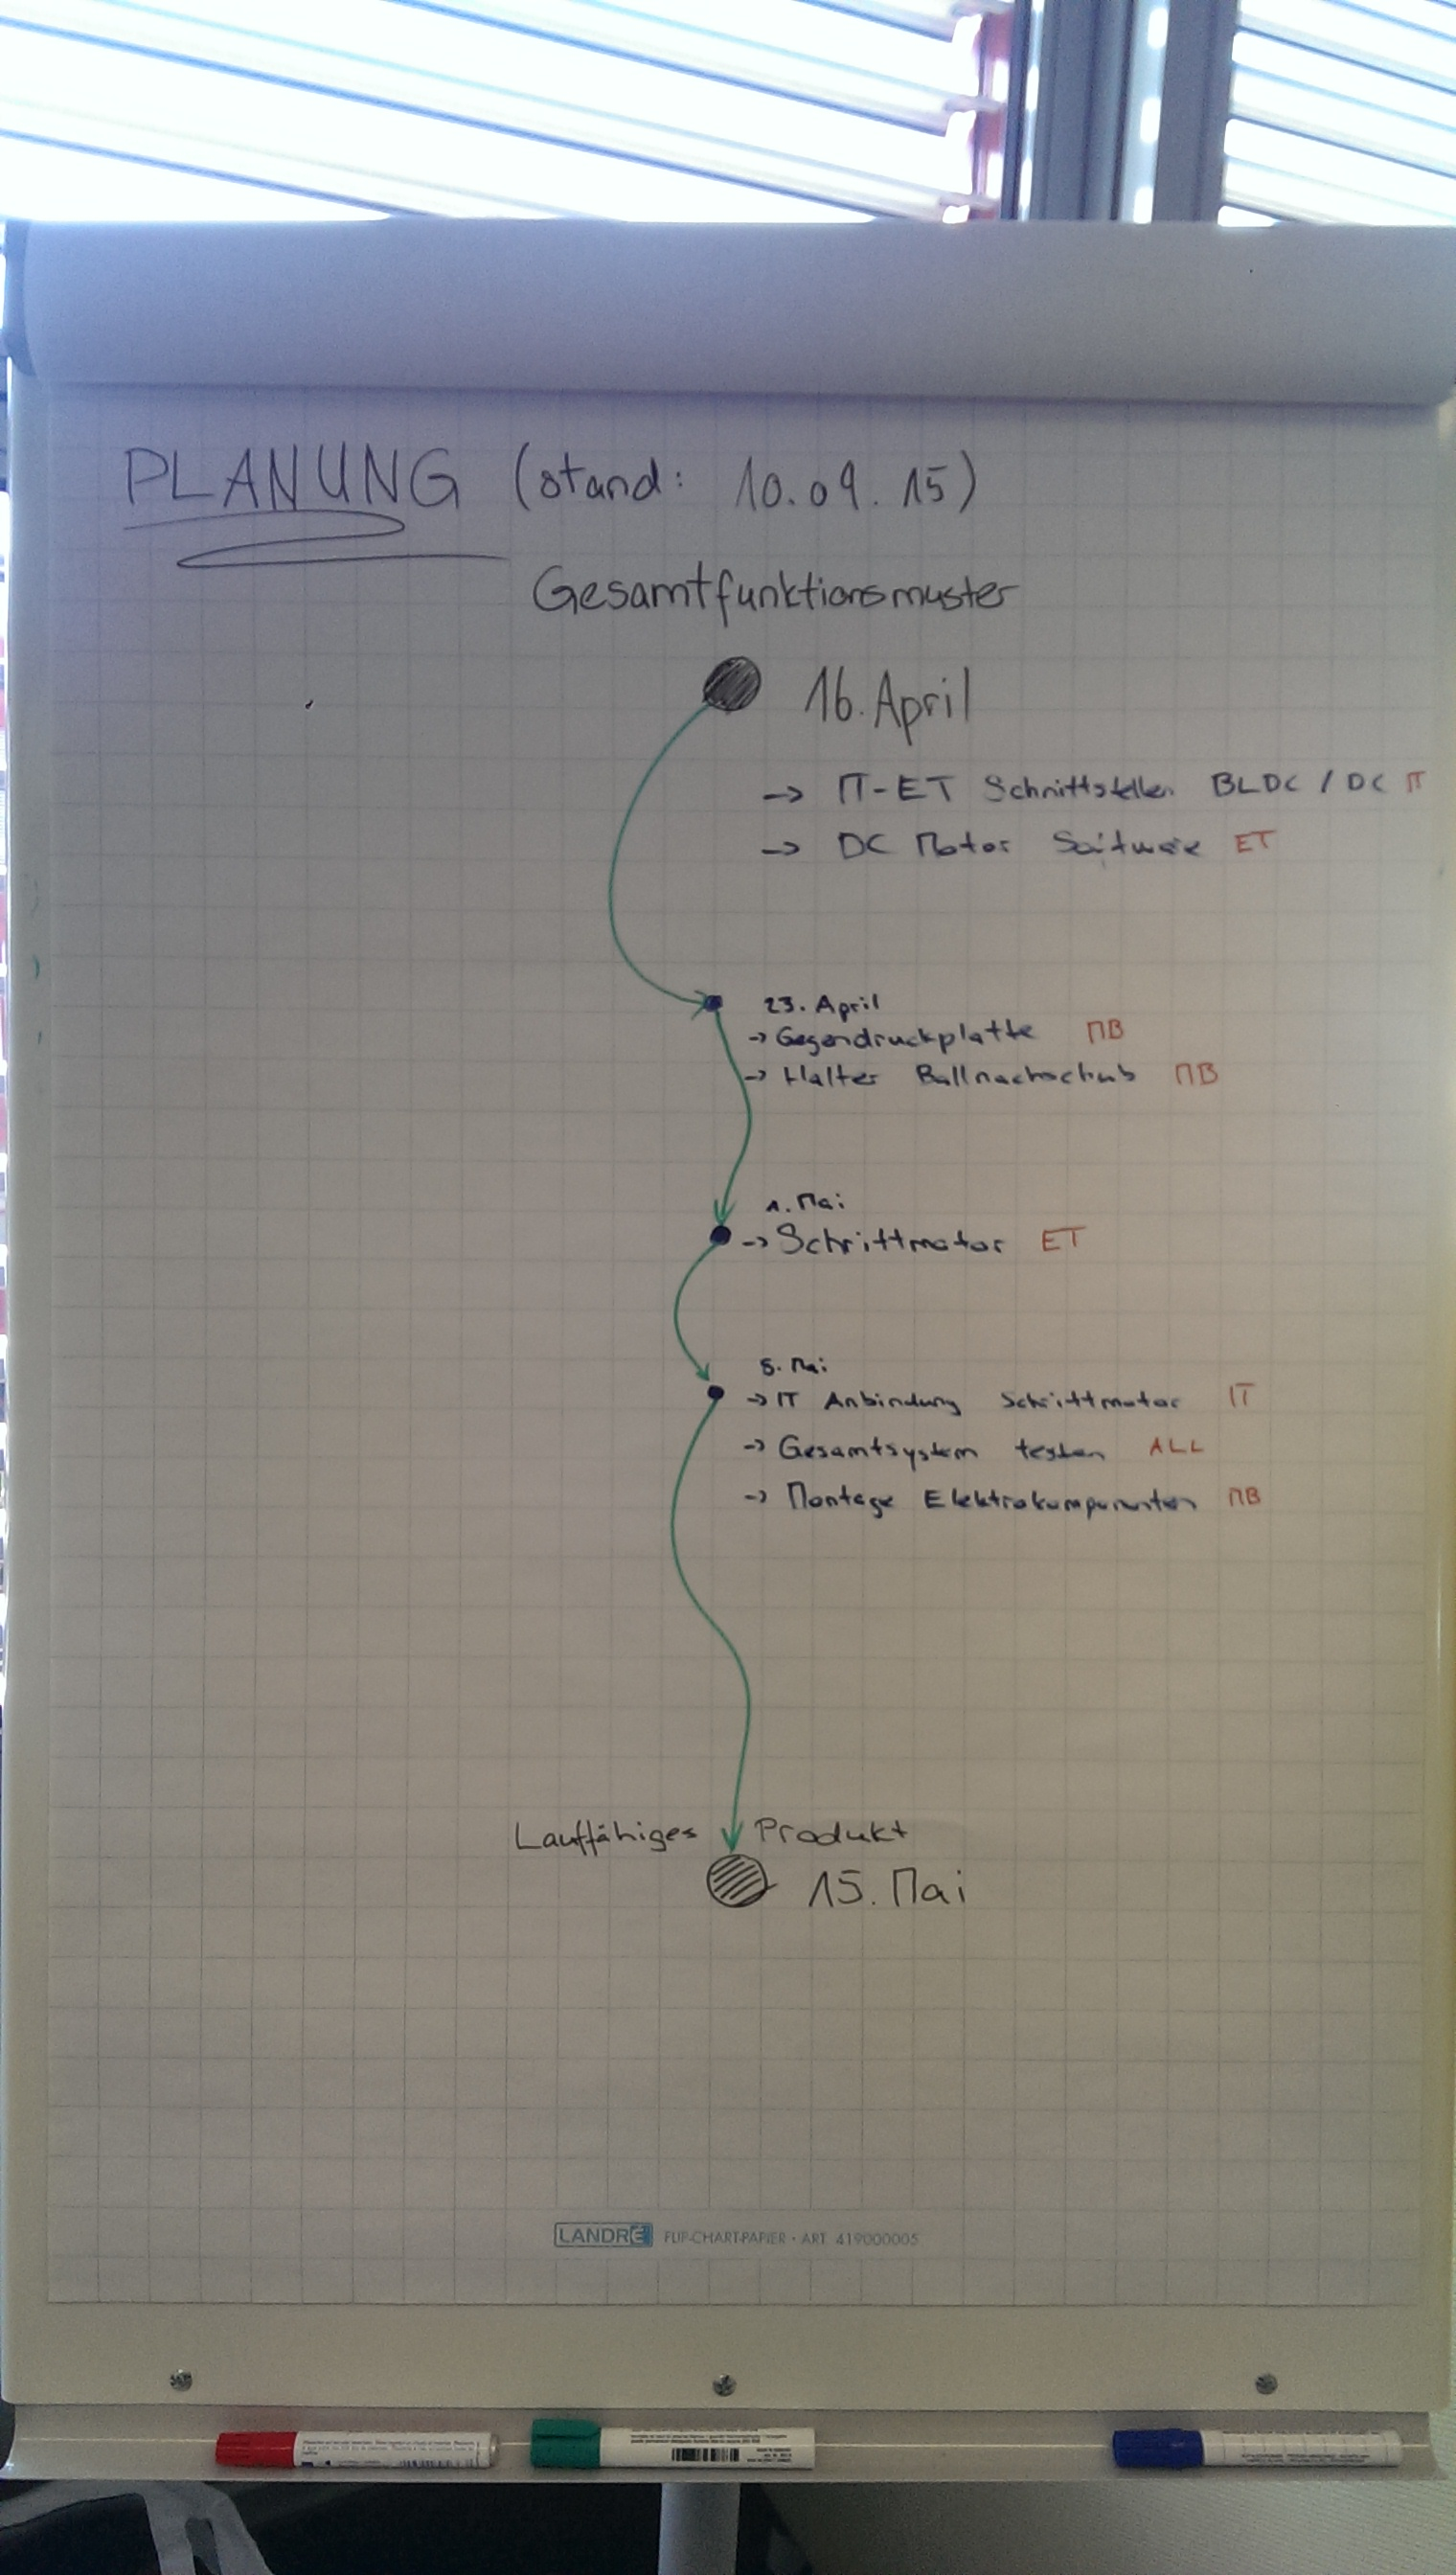
\includegraphics[width=0.6\linewidth]{../../fig/rahmenplanung-10042015}
	\caption{Rahmenplan vom 10.04.2015}
	\label{fig:rahmenplanung-10042015}
\end{figure}



\newpage
\subsection{Projektkosten}
Dem Projekt wurden 600.00 Franken zur Verfügung gestellt. In der Summe wurden 486.70 Franken davon verwendet. In der Grafik \ref{fig:kostenuebersicht} sind alle Komponenten aufgelistet.

\begin{figure}[h!]
	\centering
	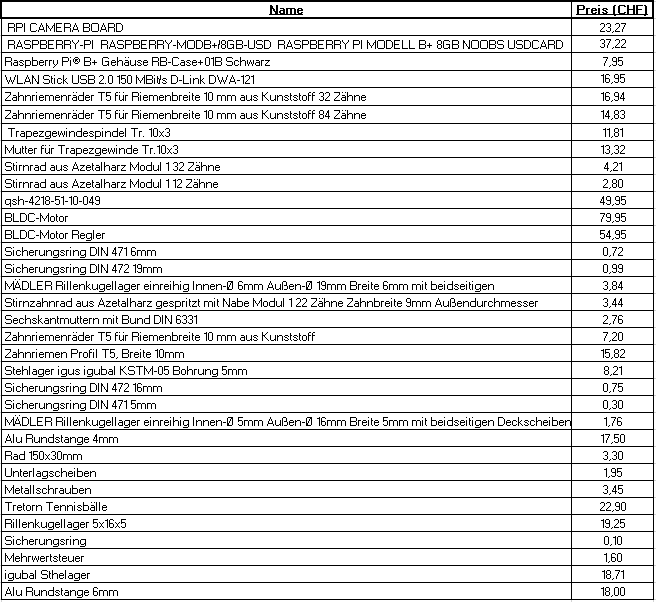
\includegraphics[width=\linewidth]{../../fig/Kosten}
	\caption{Kostenübersicht}
	\label{fig:kostenuebersicht}
\end{figure}

\newpage
\subsection{Projektrisiko}

Im Team wurden Projektrisiken evaluiert und anhand der Wahrscheinlichkeit und der entstehenden Auswirkung eingeordnet. Zusätzlich wurden Gegenmassnahmen beschrieben.

\begin{table}[h!]
	\centering
	\begin{tabular}{r || c c c c}
		häufig 		
		& \cellcolor{red} 
		& \cellcolor{red}
		& \cellcolor{red}
		& \cellcolor{red} \\
		wahrscheinlich		
		& \cellcolor{yellow} 
		& \cellcolor{yellow} 
		& \cellcolor{red}
		& \cellcolor{red} \\
		gelegentlich		
		& \cellcolor{yellow}
		& \cellcolor{yellow}
		& \cellcolor{yellow}
		& \cellcolor{red} \\
		vorstellbar		
		& \cellcolor{green}
		& \cellcolor{yellow}
		& \cellcolor{yellow}
		& \cellcolor{yellow} \\
		unwahrscheinlich	
		& \cellcolor{green}
		& \cellcolor{green}
		& \cellcolor{yellow}
		& \cellcolor{yellow} \\
		unvorstellbar		
		& \cellcolor{green}
		& \cellcolor{green}
		& \cellcolor{green}
		& \cellcolor{green} \\
		\hline
		& unwesentlich & geringfügig & kritisch & katastrophal
	\end{tabular}
	\caption{Risikoreferenz}
	\label{tab:risikoreferenz}
\end{table}


\begin{landscape}
	\begin{table}
		\begin{tabular}{|p{5cm}|c|c|p{9cm}|}
			\hline Risiko & Auswirkung & Wahrscheinlichkeit & Massnahmen \\ 
			
			\hline \rowcolor{yellow} IT, MB Projektmitglied fällt aus & geringfügig & vorstellbar & 
			- Vorzeitig über Abwesenheit informieren \newline
			- Arbeitsstand in Gruppe kommunizieren \\ 
			
			\hline \rowcolor{red} ET Projektmitglied fällt aus & katastrophal & gelegentlich & 
			- Wöchentlicher Gesundheits- und Gemütszustand rapportieren \newline
			- Aufbau Know-How in den ET Arbeiten \\
			
			\hline \rowcolor{yellow} \hline Abweichung vom Terminplan & geringfügig & vorstellbar &
			- Realistische Planung \newline
			- Aufarbeiten in Reservezeit \\ 
			
			\hline \rowcolor{yellow} \hline Fehlende Zuverlässigkeit & kritisch & unwahrscheinlich &
			- Klare Aufgabenverteilung \newline
			- Review durch Teammitglieder \\ 
			
			\hline \rowcolor{yellow} \hline Algorithmus zur Korberkennung nicht robust & kritisch & vorstellbar &
			- Gutes Unit-Testing des Algorithmus \newline
			- Früh implementieren und testen \\
			
			\hline \rowcolor{green} \hline Fehlendes Know-How IT & geringfügig & unwahrscheinlich &
			- RaspyPi früh aufsetzen \newline
			- Know-How in Python aufbauen \\ 
			
			\hline \rowcolor{yellow} \hline Integration der ET Schnittstellen in die IT Umgebung & geringfügig & wahrscheinlich &
			- Schnittstellen definieren  \\
			
			\hline \rowcolor{yellow} \hline Bälle treffen nicht präzise & kritisch & vorstellbar &
			- Früh testen \newline
			- Ballanpressdruck variieren \\ 
			
			\hline \rowcolor{yellow} \hline Stabilität beim Abwurf & kritisch & vorstellbar &
			- Mehr Gewicht montieren oder Seitenstütze \newline
			- Dicke der Wände \\ 
			
			\hline \rowcolor{yellow} \hline Falsche Dimensionierung der Motoren & kritisch & vorstellbar &
			- Motoren neu kaufen. \\
			
			\hline \rowcolor{yellow} \hline Energieversorgung: Umbau von Servernetzteilen gelingt nicht & kritisch & vorstellbar &
			- Andere Energieversorgung wählen \\ 
			
			\hline \rowcolor{yellow} \hline Schwingungen beim Abwurf & kritisch & vorstellbar &
			- Drehrad auswuchten \newline
			- Drehzahl reduzieren \newline
			- Konstruktion verstärken \\
			
			\hline \rowcolor{green} \hline Budget & geringfügig & unwahrscheinlich &
			- Budgetplanung laufend aktualisieren  \newline 
			- Planen bevor etwas eingekauft wird \\
			
			\hline \rowcolor{yellow} \hline Achse BLDC nicht stark genug & katastrophal & vorstellbar &
			- Lagerung auf der gegenüberliegenden Seite des Motors erstellen \newline
			- Trägheitsmoment Wurfrad anpassen \newline
			- Langsameres anfahren \\
			
			\hline \rowcolor{yellow} \hline BLDC überhitzt & kritisch & vorstellbar &
			- BLDC nicht im Dauerbetrieb laufen lassen \newline
			
			
			
		\end{tabular}
		\caption{Risikomanagement}
		\label{tab:risikomanagement}
	\end{table} 
\end{landscape}

\newpage

\subsection{Testplanung}

Die Tests wurden mit zwei Dokumenten durchgeführt. In einem ersten Schritt wurden alle Festanforderungen der Anforderungsliste (Anhang \ref{sec:produktanforderungen}) mit der Maschine abgeglichen und überprüft. Wurden gewisse Anforderungen nicht erfüllt, wurden diese Abweichungen dem jeweiligen Fachbereich zur Korrektur mitgeteilt. In einem nächsten Schritt wurde der Testplan (Anhang \ref{sec:testplan}) abgearbeitet. Die einzelnen Testfälle wurden von einer Person manuell durchgeführt und die Ergebnisse in einem Testprotokoll (Anhang \ref{sec:testprotokoll}) festgehalten. Zusätzlich zum Tester und dem Testdatum, wurde in einem Konfigurationsmanagement die verwendeten Softwareversionen vom Test festgehalten. Sind alle Festanforderungen erfüllt und alle Tests bestanden, gilt unsere Maschine als funktionstüchtig.

\subsection{Fazit}

Die Planung konnte grösstenteils eingehalten werden. Jedoch gab es einige Verzögerung die durch Aufwandunterschätzung und Lieferfristen der Komponenten verursacht wurde. Die Planung wurde am 10. April angepasst um den aktuellen Umständen zu entsprechen. Diese konnte ebenfalls nicht vollständig eingehalten werden. Besonders die Elektrotechnik stand unter Zeitdruck, da nur ein Projektmitglied das nötige Fachwissen besass.
Die Projektrisiken konnten ohne grosse Mühe bewältigt werden, da nur sehr kleine Probleme auftraten.
Von diesen gab es jedoch mehrere, welche summiert zu Verzögerungen führten, da jedes neue Bauteil eingekauft oder angefertigt werden musste. Dies verschob die Funktionstests um zwei Wochen.
Der Schrittmotor funktionierte ebenfalls zwei Wochen nach der angepassten Planung.
Die Kosten blieben hingegen von Beginn an moderat und passten ins vorgesehene Budget.
